% ------------------------------------------------------------------
\documentclass[12 pt]{article}
\pagestyle{plain}
\pagenumbering{arabic}

\setlength{\parindent}{10 mm}
\setlength{\parskip}{12 pt}

% Nimbus Sans font should be reasonably legible
\usepackage{helvet}
\renewcommand{\familydefault}{\sfdefault}

% Section header spacing
\usepackage{titlesec}
\titlespacing\section{0pt}{12pt plus 4pt minus 2pt}{0pt plus 2pt minus 2pt}
\titlespacing\subsection{0pt}{12pt plus 4pt minus 2pt}{0pt plus 2pt minus 2pt}
\titlespacing\subsubsection{0pt}{12pt plus 4pt minus 2pt}{0pt plus 2pt minus 2pt}

\usepackage{amsmath}
\usepackage{amssymb}
\usepackage{graphicx}
\usepackage{verbatim}    % For comment
\usepackage[paper=a4paper, marginparwidth=0 cm, marginparsep=0 cm, top=2.5 cm, bottom=2.5 cm, left=3 cm, right=3 cm, includemp]{geometry}
\usepackage[pdftex, pdfstartview={FitH}, pdfnewwindow=true, colorlinks=true, citecolor=blue, filecolor=blue, linkcolor=blue, urlcolor=blue, pdfpagemode=UseNone]{hyperref}

%\usepackage{amsfonts}
%\usepackage{float}
\usepackage{framed,color}
\usepackage{fancybox}
\usepackage{varwidth}
\definecolor{shadecolor}{rgb}{1,0.8,0.3}
\usepackage[framemethod=tikz]{mdframed}
% ------------------------------------------------------------------



% ------------------------------------------------------------------
% Shortcuts
\newcommand{\cE}{\ensuremath{\mathcal E} }
\newcommand{\cF}{\ensuremath{\mathcal F} }
\newcommand{\Nbb}{\ensuremath{\mathbb N} }
\newcommand{\cO}{\ensuremath{\mathcal O} }
\newcommand{\Rbb}{\ensuremath{\mathbb R} }
\newcommand{\al}{\ensuremath{\alpha} }
\newcommand{\be}{\ensuremath{\beta} }
\newcommand{\De}{\ensuremath{\Delta} }
\newcommand{\si}{\ensuremath{\sigma} }
\newcommand{\om}{\ensuremath{\omega} }
\newcommand{\Om}{\ensuremath{\Omega} }
\newcommand{\lra}{\ensuremath{\longrightarrow} }
\newcommand{\Lra}{\ensuremath{\Longrightarrow} }
\newcommand{\llra}{\ensuremath{\longleftrightarrow} }
\newcommand{\X}{\ensuremath{\!\times\!} }
\newcommand{\vev}[1]{\ensuremath{\left\langle #1 \right\rangle} }
\newcommand{\fig}[1]{Figure~\ref{#1}}
\newcommand{\TODO}[1]{\textcolor{red}{\textbf{#1}}}
% ------------------------------------------------------------------



% ------------------------------------------------------------------
\begin{document}
\begin{center}
  {\LARGE \textbf{MATH327: Statistical Physics}} \\[6 pt]
  \textbf{David Schaich \qquad\qquad\qquad\qquad Spring 2021} \\[48 pt]
  {\LARGE LECTURE \ NOTES} \\[6 pt]
  Last modified 8 January 2021
\end{center}
\renewcommand{\contentsname}{}
\setcounter{tocdepth}{1}
\tableofcontents
% ------------------------------------------------------------------



% ------------------------------------------------------------------
\newpage
\setcounter{section}{0}
\addcontentsline{toc}{section}{Module information}
\section*{Module information}
\subsection*{Coordinator}
\begin{description}
  \setlength{\itemsep}{1pt}
  \setlength{\parskip}{0pt}
  \setlength{\parsep}{0pt}
  \item[\qquad] Dr David Schaich
  \item[\qquad] Mathematics Building Room 124 (Theoretical Physics Wing)
  \item[\qquad] \href{mailto:david.schaich@liverpool.ac.uk}{david.schaich@liverpool.ac.uk}
  \item[\qquad] \href{http://www.davidschaich.net}{www.davidschaich.net} \\
  \item[\qquad] Office hours: \TODO{...} and by request via \href{https://calendly.com/daschaich}{calendly.com/daschaich}
\end{description}
% ------------------------------------------------------------------



% ------------------------------------------------------------------
\subsection*{Logistics, lecture notes, and learning strategy}
All resources for this module are gathered at its Canvas site.
\TODO{notes-driven delivery with recorded introductions and take-aways...}
\TODO{notes have gaps --- attempt to fill these in as exercise, which we will review during synchronous sessions and (depending on demand) through supplemental video...}
In addition to these lecture notes, these resources include explanatory videos, sample problems \TODO{and more...}
\TODO{...weekly introductory overview and take-away...}
\TODO{...possible supplements by demand/survey...} % TODO: Need to be provided a week in advance?...
\TODO{...can supplement with recorded lectures from last year on stream.liv.ac.uk...}

\TODO{...numbered equations and colored boxes...}

\TODO{...module organized in terms of statistical ensembles...}
\TODO{...focusing on systems whose constituents (which may be particles, balls, spins or other objects) do not interact with each other...}

\subsubsection*{Expected background}
\TODO{Quantum and combinatorics not assumed... do expect binomial coefficients and gaussian integrals}

\subsubsection*{Version control and co-creation}
The \LaTeX\ source for these lecture notes is kept under version control at \\
\centerline{\href{https://github.com/daschaich/MATH327_2021}{github.com/daschaich/MATH327\_2021}}
If any changes need to be made to these notes during the term (to correct mistakes or add supplemental information), the GitHub interface provides an easy way to see what changed and when.
In addition, you are also welcome to use GitHub to report issues and create pull requests to address them.
Such co-creation is entirely optional.
If you are interested in learning more about version control with \texttt{git}, the \href{https://software-carpentry.org}{Software Carpentry} project provides free resources at \\
\centerline{\href{https://swcarpentry.github.io/git-novice/}{swcarpentry.github.io/git-novice/}}
% ------------------------------------------------------------------



% ------------------------------------------------------------------
\subsection*{Assessment and academic integrity}
The assessment workload has also been kept the same as last year, but in light of this year's hybrid teaching and learning approach the weighting of assignments has been spread more evenly across the term to avoid a high-stakes final assessment.
The following deadlines for the in-term assignments have been coordinated within the Department to minimize pile-up: \\[-24 pt]
\begin{description}
  \item[15\%] A homework assignment covering weeks 1--3, due \TODO{Friday, 5 March (TBC)}
  \item[20\%] A computer-based project divided into two equally weighted parts, the first due \TODO{Friday, 19 March (TBC)} and the second due \TODO{Friday, 16 April (TBC}
  \item[15\%] A homework assignment covering weeks 4--8, due \TODO{Friday, 30 April (TBC)}
  \item[50\%] A final assessment to be centrally scheduled within the period 17 May through 4 June
\end{description}

Because the computer-based project will be done remotely, rather than in a computer lab on campus, you are free to complete it using the programming language of your choice.
Training in the necessary programming concepts will be provided using \href{https://www.python.org}{Python}, the free programming language recommended for the project.
If you have difficulty setting up Python on your device, you can run it for free online at \href{https://repl.it/languages/python3}{repl.it}.
(Make sure to keep a copy of the code to submit for assessment!)
Alternative languages could include \href{https://en.wikipedia.org/wiki/C_(programming_language)}{C}, \href{https://www.r-project.org}{R}, or even \href{https://matlab.mathworks.com}{MATLAB} (through the University's site license).
Maple may struggle to handle parts of the project.

I encourage you to discuss the in-term assignments with each other, since discussing and debating concepts and procedures is a very effective way to learn.
The examination must be done on your own, and your submissions for all assignments must be your own work representing your own understanding.
Clear and neat presentations of your workings and the logic behind them will contribute to your mark.
It is unacceptable to copy solutions in part or in whole from other students (current or prior) or from other sources (commercial or otherwise).
Should you make use of resources beyond the module materials, these must be explicitly referenced in your work.

By now you should have successfully passed the Academic Integrity Tutorial and Quiz to affirm that you have read and understood the Academic Integrity Policy detailed in Appendix L of the Code of Practice on Assessment.
If you have any questions about what is or is not acceptable under this policy, please ask me or Departmental Assessment Officer Kamila Zychaluk.
In all cases, the spirit of the Academic Integrity Policy should take precedence over legalistic convolutions of the text.
% ------------------------------------------------------------------



% ------------------------------------------------------------------
\subsection*{Additional resources}
The lists of further reading below provide some optional additional resources that may be helpful.
Hyperlinks lead either to the resource itself or to the corresponding record page in our library.

\noindent\textbf{These books and lecture notes are roughly at the level of this module:} \\[-24 pt]
\begin{enumerate}
  \item David Tong, \href{https://www.damtp.cam.ac.uk/user/tong/statphys.html}{\textit{Lectures on Statistical Physics}} (2012), \\ www.damtp.cam.ac.uk/user/tong/statphys.html
  \item Daniel V.~Schroeder, \textit{An Introduction to Thermal Physics} (first edition, 2000)
  \item C.~ Kittel and H.~Kroemer, \textit{Thermal Physics} (second edition, 1980)
  \item F.~Reif, \textit{Fundamentals of Statistical and Thermal Physics} (first edition, 1965)
\end{enumerate}

\noindent\textbf{These books are more advanced and more specialized, but can be useful to consult concerning specific questions or topics:} \\[-24 pt]
\begin{enumerate}
  \setcounter{enumi}{4}
  \item Weinan E, Tiejun Li and Eric Vanden-Eijnden, \textit{Applied Stochastic Analysis} (first edition, 2019)
  \item R.~K.~Pathria, \textit{Statistical Mechanics} (second edition, 1996)
  \item Sidney Redner, \textit{A Guide to First-Passage Processes} (first edition, 2007)
  \item Pavel L.~Krapivsky, Sidney Redner and Eli Ben-Naim, \textit{A Kinetic View of Statistical Physics} (first edition, 2010)
  \item Kerson Huang, \textit{Statistical Mechanics} (second edition, 1987)
  \item Michael Plischke and Birger Bergersen, \textit{Equilibrium Statistical Physics} (third edition, 2005)
  \item L.~D.~Landau and E.~M.~Lifshitz, \textit{Statistical Physics, Part 1} (third edition, 1980)
\end{enumerate}

\noindent\textbf{Maple and MATLAB resources:} \\[-24 pt]
\begin{enumerate}
  \setcounter{enumi}{11}
  \item Ian Thompson, \href{https://library.liv.ac.uk/record=b4395758~S8}{\textit{Understanding Maple}} (ebook edition, 2017) \\
        Related videos: \href{https://stream.liv.ac.uk/4k67bdzt}{\textit{Running Maple for the first time}} (stream.liv.ac.uk/4k67bdzt) \\
        \textcolor{white}{Related videos:} \href{https://stream.liv.ac.uk/7pjge23a}{\textit{Configuring Maple}} (stream.liv.ac.uk/7pjge23a)
  \item Stormy Attaway, \textit{MATLAB: A Practical Introduction to Programming and Problem Solving} (third edition, 2013)
  \item B.~Barnes and G.~R.~Fulford, \textit{Mathematical Modelling with Case Studies: Using Maple and MATLAB} (third edition, 2014)
\end{enumerate}

Finally, there is a vast constellation of purely online resources, such as \href{https://en.wikipedia.org/wiki/Statistical_physics}{Wikipedia}.
These are often fine places to \emph{start} learning about a subject, but may be terrible places to \emph{stop}.
% ------------------------------------------------------------------



% ------------------------------------------------------------------
\newpage
\setcounter{section}{1}
\section*{Week 1: Central limit theorem and diffusion}
\addcontentsline{toc}{section}{Week 1: Central limit theorem and diffusion}

\subsection*{Introductory remarks: What is Statistical Physics?}
Mathematical sciences such as physics aim to determine the laws of nature and understand how these govern experimental observations---both in everyday circumstances and under extreme conditions.
This mathematical understanding is typically guided by reproducing a set of observations, with the resulting framework then used to make predictions for other ``observables''.

Over the past few centuries this process has been tremendously successful, with theoretical physics accurately predicting experimental and observational results from sub-atomic through to extra-galactic scales.
Modern physics labs can create a vacuum better than in outer space and the coldest temperatures in the known universe, as well as going to the other extreme to reach temperatures of millions of degrees and pressures millions of times atmospheric pressure at sea level.
Amazingly, many aspects of these realms of physics can be theoretically described by mathematics developed centuries ago.\footnote{Eugene Wigner's famous article, ``\href{https://en.wikipedia.org/wiki/The_Unreasonable_Effectiveness_of_Mathematics_in_the_Natural_Sciences}{The Unreasonable Effectiveness of Mathematics in the Natural Sciences}'' (1960), and subsequent work in the philosophy of physics, elaborates on why this may be considered `amazing'.  These lecture notes will not comment extensively on philosophy.}

The domain of \textbf{statistical physics} is one in which simple mathematical principles enable amazing predictive capabilities.
Initially developed in the nineteenth century, statistical physics remains a core component of modern physics, and will retain this position in years to come.
The foundations of statistical physics lie in the use of probability theory to mathematically describe experimental observations and corresponding laws of nature that involve stochastic randomness rather than being perfectly predictable.

The lack of perfect predictability in statistical physics is a matter of practicality rather than one of principle.
It results from working with a large number of degrees of freedom (i.e., a large number of independent objects such as particles or balls).
For example, Avogadro's number $N_A \approx 6.022\times 10^{23}$ is the large number of molecules in everyday amounts of familiar substances---about 18~grams of water or about 22~litres of air at sea-level atmospheric pressure ($\approx$$101$~kPa). % 22.4 litres for 1atm=101.325~kPa, 22.71 litres for 100~kPa at $O^{\circ}$~C
Specifying the positions and velocities of $\sim$$10^{23}$ objects would require far more information than could be stored even in the memory of the biggest existing supercomputers.
Statistical physics instead produces simple mathematical descriptions of large-scale properties such as temperature, pressure and diffusion, which are generally of such outstanding quality that the underlying `randomness' is effectively undetectable.

Historically, the difficulty detecting the stochastic processes underlying such \textit{thermodynamic} properties made it challenging to convince skeptics that atoms and molecules really existed.
Ludwig Boltzmann, a prominent early developer of statistical physics, endured a constant struggle to defend his ideas, which likely contributed to his deteriorating mental health and eventual suicide in 1906.
A crucial advance to convincingly establish the existence of atoms was Albert Einstein's use of statistical physics to explain the observed ``\href{https://en.wikipedia.org/wiki/Brownian_motion}{Brownian motion}'' of particles suspended in fluids---this work was part of Einstein's ``miracle year'' in 1905, along with special relativity and early contributions to quantum physics.
More modern applications of statistical physics include explaining why stars don't collapse under the `weight' of their own gravity, and identifying effects of dark matter in temperature fluctuations observable in the \textit{cosmic microwave background} lingering from the early years of the universe.

For this week we will focus on some of the foundational mathematics that will underlie our later development and application of statistical ensembles.
Looking back to Boltzmann's times, we can consider the following question one of his opponents might have asked:
\textit{If the pressure of a gas in a container results from molecules stochastically colliding with the walls of that container and pushing them out, then how can the pressure be so stable and reproducible, rather than itself fluctuating stochastically?}
The mathematical answer lies in the \textbf{law of large numbers} and the \textbf{central limit theorem}, which this week we will learn and apply to the physics of diffusion in one dimension.
% ------------------------------------------------------------------



% ------------------------------------------------------------------
\subsection{Probability foundations}
Let's begin by placing some familiar everyday concepts into a more formal mathematical framework through the following definitions: \\[-24 pt]
\begin{itemize}
  \item A (random) \textbf{experiment} \cE involves setting up, manipulating and/or observing some (physical or hypothetical) system with some element of randomness.
        Flipping a coin is a simple random experiment.
        In the context of the statistical ensembles that will be the focus of this module, the typical experiment will be simply allowing a collection of particles to evolve in time, subject to certain constraints.
  \item Each time an experiment is performed, the world comes out in some \textbf{state} $\om$.
        The definition of the experiment and the state must include all objects of interest, and may include more besides.
        When flipping a coin, for example, the full state could contain information not only about the final orientation of the coin, but also about its position---did it land on the floor or on a cat?
  \item The \textbf{set of all states} \Om collects all possible states \om that the given experiment \cE can produce, and is therefore intricately tied to \cE itself.
  \item We are generally not interested in all aspects of the full state $\om$.
        For example, we won't care where a flipped coin lands.
        Instead we're typically only interested in whether it lands heads up or tails up---and we may want to set aside any state that doesn't cleanly map on to those options.
        The \textbf{measurement} $X(\om)$ extracts and quantifies this information, acting as a function that maps the state \om to a number that we can mathematically manipulate.
        If we repeat a fixed experiment \cE many times and carry out the measurement $X$ on each resulting state $\om$, we will obtain a sequence of numbers $X(\om)$ that behave as a \textit{random variable}.
  \item Acting with the measurement $X$ on all of the possible states in the set $\Om$ defines the \textbf{set of all outcomes} (or \textbf{outcome space}) $A$:
        \begin{equation*}
          X: \Om \to A.
        \end{equation*}
        That is, $A$ collects all possible measurement results that the given experiment \cE and measurement $X$ can produce.
        $A$ can be finite, countably infinite, or uncountably infinite (i.e., continuous).
  \item Finally, defining an \textbf{event} to be any subset of the set of all outcomes $A$, we further group these subsets together to define a \textbf{set of events} $\cF$.
\end{itemize}

Let's consider some \textbf{examples} to clarify these definitions.
With an experiment of rolling a six-sided die and measuring the number ($1$--$6$) that comes out on top, what is the set of all outcomes $A$, and what additional information could be present in the set of all states $\Om$?
\begin{mdframed}
  \ \\[100 pt]
\end{mdframed}
What is the outcome space $A$ if we toss a coin four times and measure whether it lands heads up ($H$) or tails up ($T$)?
\begin{mdframed}
  \ \\[100 pt]
\end{mdframed}
\newpage % WARNING: FORMATTING BY HAND
\noindent What information would characterize a state \om for a gas of $6\X 10^{23}$ argon atoms in a container?
\begin{mdframed}
  \ \\[100 pt]
\end{mdframed}

We can generalize the concept of measurement by introducing a unique number as a \textit{label} to characterize each state \om in the set $\Om$.
This would provide a label function $L(\om)$ as a random variable.
Our condition of uniqueness makes $L(\om)$ isomorphic, so that the label can be used interchangeably with the full state,
\begin{equation*}
  \om \llra L(\om).
\end{equation*}
While the measurements $X(\om)$ we consider will generally not produce a unique number for each $\om$, we will design them (as best we can) precisely to remove irrelevant information that doesn't interest us.
Ignoring that irrelevant information leaves us free to interchange the set of outcomes $A$ for the set of states $\Om$, which we will do from now on.
(Some textbooks may never distinguish between $A$ vs \Om in the first place, though this can be a source of confusion.)

We are now prepared for the final foundational definition in this section, the \textbf{probability} $P$ that an event in the set \cF has of occurring.
Mathematically, $P$ is a \textit{measure function},
\begin{equation*}
  P: \cF \to [0, 1],
\end{equation*}
which must satisfy the following two requirements: \\[-24 pt]
\begin{enumerate}
  \item The probability of a countable union of mutually exclusive events must equal the countable sum of the probabilities of each of these events.
  \item The probability of the outcome space ($\cF = A$) must equal $1$ (even if $A$ is uncountable).
        This simply means that the experiment \cE must produce an outcome.
        If no outcome were produced, it would not make sense to say that the experiment had occurred.
\end{enumerate}
Combining the outcome space, event space and probability measure gives us a \textit{probability space} $(A, \cF, P)$.

For \textbf{example}, consider an experiment that can only produce $N$ possible states as outcomes, so that
\begin{equation*}
  \Om = \left\{\om_1, \om_2, \cdots, \om_N\right\}.
\end{equation*}
If two states are identical, $\om_i = \om_j$, they must produce the same measurements $X(\om_i) = X(\om_j)$, which implies the contra-positive
\begin{equation*}
  X(\om_i) \ne X(\om_j) \qquad \Lra \qquad \om_i \ne \om_j.
\end{equation*}
On the other hand, as described above, it is possible to have $X(\om_i) = X(\om_j)$ even when $\om_i \ne \om_j$.
This means that the size $n$ of the outcome space $A$ may be smaller than the size of $\Om$, $n \leq N$.
We can write
\begin{equation*}
  A = \left\{X_1, X_2, \cdots, X_n\right\},
\end{equation*}
where each $X_{\al}$ is distinct and its index does \textit{not} necessarily correspond to that on $\om_i$.
We can take the individual $X_{\al}$ themselves to be the events we're interested in, with an overall event space
\begin{equation*}
  \cF = \left\{X_1, X_2, \cdots, X_n\right\} = A.
\end{equation*}
These events are all mutually exclusive by construction, so if we assign them probabilities
\begin{equation*}
  P(X_{\al}) \equiv p_{\al} \qquad \mbox{for } \al = 1, \cdots, n,
\end{equation*}
then the above requirements on probabilities demand that for any $\al \ne \be$ we have
\begin{align*}
  P(X_{\al} \mbox{ or } X_{\be}) & = p_{\al} + p_{\be} \\
  P(X_1 \hbox{ or } X_2 \hbox{ or } \cdots \mbox{ or } X_n) & = \sum_{\al = 1}^n p_{\al} = 1.
\end{align*}

Similarly choosing an event space $\cF = A$ for the six-sided die considered in an earlier gap, what are the probabilities $p_1$ through $p_6$ that result from assuming the die is \textit{fair} (meaning that each outcome is equally probable)?
\begin{mdframed}
  \ \\[100 pt]
\end{mdframed}
\newpage % WARNING: FORMATTING BY HAND
\noindent Again taking $\cF = A$ for the case of tossing a coin four times, what are the probabilities $p_{\al}$ that result from assuming the coin is fair?
If we instead consider the event space
\begin{equation*}
  \cF = \left\{\mbox{equal number of } H \mbox{ and } T, \mbox{ different numbers of } H \mbox{ and } T\right\},
\end{equation*}
what are the probabilities $p_{\text{equal}}$ and $p_{\text{diff}}$ for the two events in this $\cF$?
\begin{mdframed}
  \ \\[100 pt]
\end{mdframed}

\begin{minipage}{0.4\textwidth}
  \begin{center}
    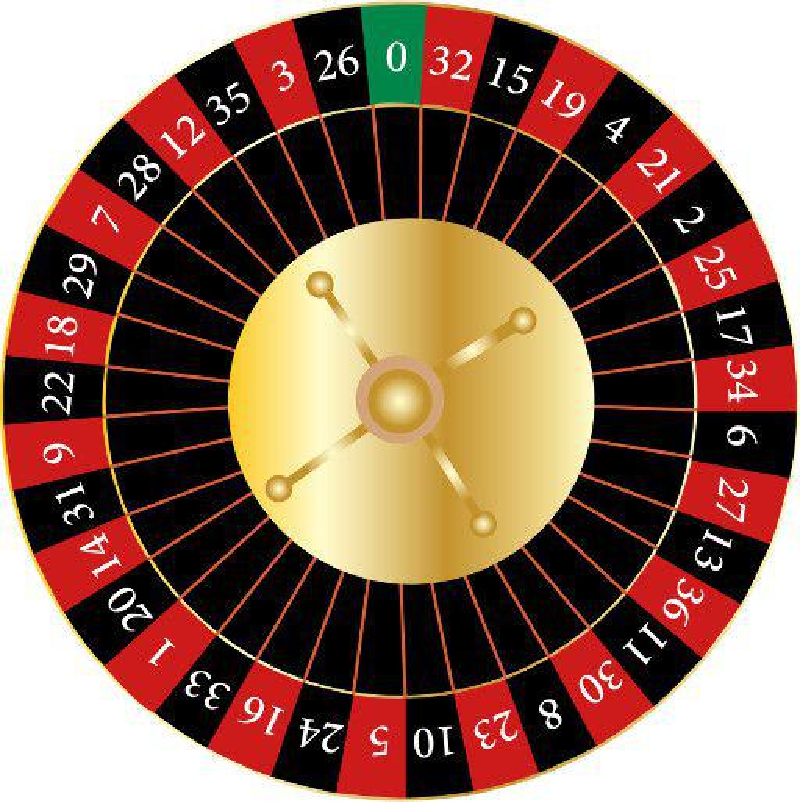
\includegraphics[width=0.75\textwidth]{figs/roulette.pdf} \\
    \href{https://www.vecteezy.com/vector-art/658761-casino-roulette-wheel}{Source}
  \end{center}
\end{minipage}%
\begin{minipage}{0.5\textwidth}
  The standard European roulette wheel shown to the left has 37 pockets labelled ``0'' through ``36''.
  18 of these pockets are coloured red, 18 are coloured black and 1 (pocket ``0'') is coloured green.
\end{minipage}

\noindent What is the outcome space $A$ for a spin of the roulette wheel?
With $\cF = A$, what are the probabilities $p_{\al}$ for a fair wheel?
With
\begin{equation*}
  \cF = \left\{\mbox{ball in a red pocket, ball in a black pocket, ball in the green pocket}\right\},
\end{equation*}
what are the corresponding probabilities $p_{\text{red}}$, $p_{\text{black}}$ and $p_{\text{green}}$?
\begin{mdframed}
  \ \\[100 pt]
\end{mdframed}

We conclude this section with two \textbf{comments} on 
\TODO{...}
% ------------------------------------------------------------------



% ------------------------------------------------------------------
\newpage
\setcounter{section}{2}
\section*{Week 2: Micro-canonical ensemble}
\addcontentsline{toc}{section}{Week 2: Micro-canonical ensemble}
% ------------------------------------------------------------------



% ------------------------------------------------------------------
\newpage
\setcounter{section}{3}
\section*{Week 3: Canonical ensemble}
\addcontentsline{toc}{section}{Week 3: Canonical ensemble}
% ------------------------------------------------------------------



% ------------------------------------------------------------------
\newpage
\setcounter{section}{4}
\section*{Week 4: Ideal gases}
\addcontentsline{toc}{section}{Week 4: Ideal gases}
% ------------------------------------------------------------------



% ------------------------------------------------------------------
\newpage
\setcounter{section}{5}
\section*{Week 5: Thermodynamic cycles}
\addcontentsline{toc}{section}{Week 5: Thermodynamic cycles}
% ------------------------------------------------------------------



% ------------------------------------------------------------------
\newpage
\setcounter{section}{6}
\section*{Week 6: Grand-canonical ensemble}
\addcontentsline{toc}{section}{Week 6: Grand-canonical ensemble}
% ------------------------------------------------------------------



% ------------------------------------------------------------------
\newpage
\setcounter{section}{7}
\section*{Week 7: Quantum statistics}
\addcontentsline{toc}{section}{Week 7: Quantum statistics}
% ------------------------------------------------------------------



% ------------------------------------------------------------------
\newpage
\setcounter{section}{8}
\section*{Week 8: Quantum gases of bosons}
\addcontentsline{toc}{section}{Week 8: Quantum gases of bosons}
% ------------------------------------------------------------------



% ------------------------------------------------------------------
\newpage
\setcounter{section}{9}
\section*{Week 9: Quantum gases of fermions}
\addcontentsline{toc}{section}{Week 9: Quantum gases of fermions}
% ------------------------------------------------------------------



% ------------------------------------------------------------------
\newpage
\setcounter{section}{10}
\section*{Week 10: Interacting systems}
\addcontentsline{toc}{section}{Week 10: Interacting systems}
% ------------------------------------------------------------------



% ------------------------------------------------------------------
\newpage
\setcounter{section}{11}
\section*{Week 11: Synthesis and broader applications}
\addcontentsline{toc}{section}{Week 11: Synthesis and broader applications}
% ------------------------------------------------------------------



% ------------------------------------------------------------------
\end{document}
% ------------------------------------------------------------------
